\documentclass[conference]{IEEEtran}
\IEEEoverridecommandlockouts
% The preceding line is only needed to identify funding in the first footnote. If that is unneeded, please comment it out.
\usepackage{cite}
\usepackage{amsmath,amssymb,amsfonts}
\usepackage{algorithmic}
\usepackage{graphicx}
\usepackage{textcomp}
\usepackage{slashbox}
\usepackage{xcolor}
\def\BibTeX{{\rm B\kern-.05em{\sc i\kern-.025em b}\kern-.08em
    T\kern-.1667em\lower.7ex\hbox{E}\kern-.125emX}}
\begin{document}

\title{Network APIs and Programmable Networks: 
}

\author{\IEEEauthorblockN{Elwan Yassin, Fischer Carmen, Fuhrmann Martin}
\textit{FH Campus Wien}\\
Computer Science and Digital Communications \\
Vienna, Austria}


\maketitle

\section{Introduction}
In traditional IP networks, the control plane (that decides how to handle network traffic) and the data plane (that forwards traffic according to the decisions made by the control plane) are tightly coupled, embedded in the same networking devices, and the whole structure is highly decentralized. Network operators need to configure each individual network device separately using low-level and often vendor-specific commands. This is the fundamental reason why traditional networks are rigid, and complex to manage and control. \\ \\
*picture of conventional network
\\ \\
Software-defined networking (SDN) aims to overcome that limitations by separating the network's control logic from the underlying routers and switches that forward the traffic. With the separation of the control and data planes, network switches become simple forwarding devices and the control logic is implemented in a logically centralized controller (SDN controller).
This separation is key to the desired flexibility, breaking the network control problem into tractable pieces, and making it easier to create and introduce new abstractions in networking. The separation of the control plane and the data plane can be realized by means of a well-defined programming interface (API) between the switches and the SDN controller. The controller exercises direct control over the state in the data plane elements via this API, as depicted in \ref{fig:sdn}. \\

This centralization of network control introduces the ability to program the network, to be dynamically configured and managed through software applications, enhancing flexibility and efficiency. SDN's can also offer an API to application developers, a so-called northbound interface to be used for developing new applications. Through this network architecture, new services can be offered, such as authentication, location, billing, messaging, network quality, privacy/security, etc.

\cite{6994333}
\begin{figure}[htbp]
	\centering
	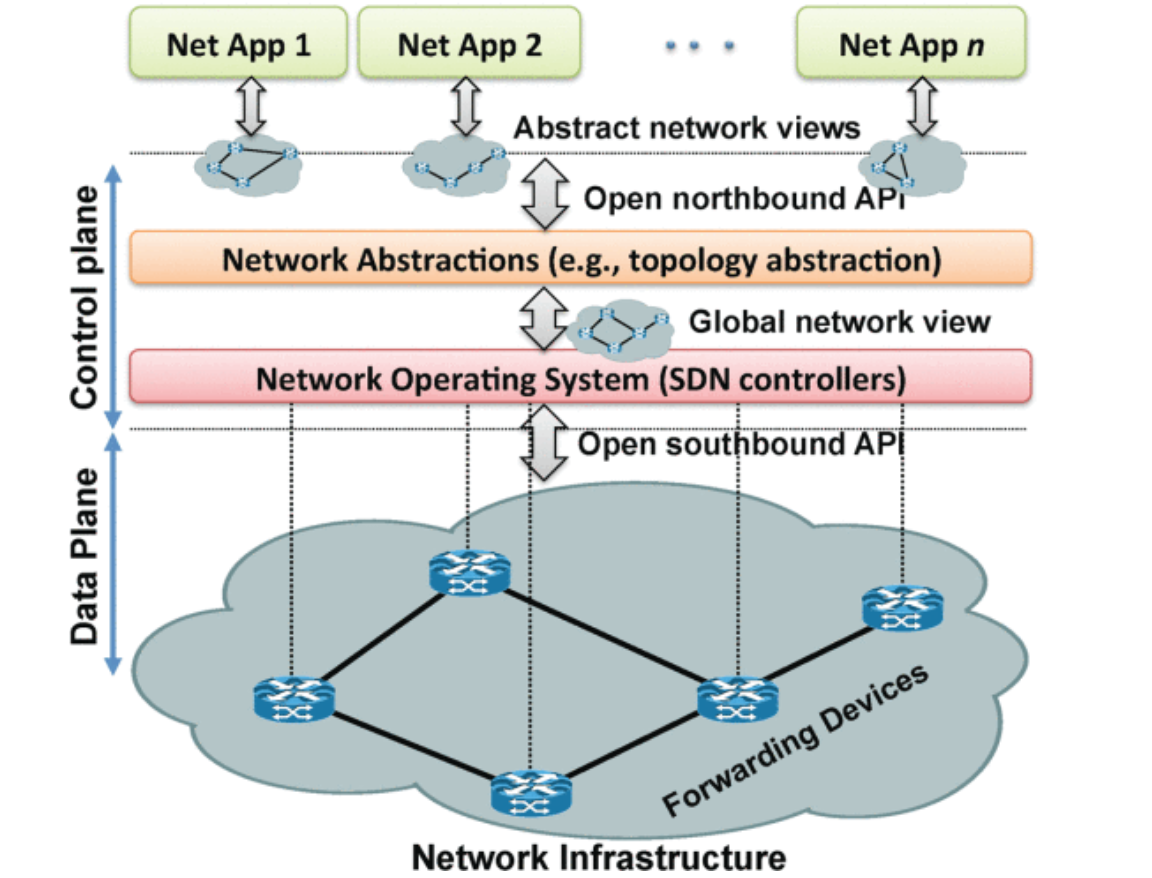
\includegraphics[width=0.8\linewidth]{pics/sdn_architecture.png}
	\caption{SDN architecture}
	\label{fig:sdn}
\end{figure}

\section{Network APIs}\label{AA}

\subsection{Billing}
\textbf{Monitoring Applications:} SDN controllers host network monitoring applications or services that collect and analyze traffic data.

\textbf{Flow Statistics:} Monitoring applications query switch flow tables to retrieve flow statistics (e.g., packet count, byte count) for tracking user traffic.

\textbf{Integration with Identity Systems:} SDN controllers integrate with identity management systems to associate network traffic with specific users or devices.

\section{Device Localisation}

\section{Identity Managment}
The CAMARA project is currently in the process of defining an API for Identity and Consent Managment. This API the then can be used to for other CAMARA APIs to fully comply with GDPR regulations, another use of this API can be to manage consent through the life cycle. Naturally for these the the identity of the end user and subscriber must be determined, as both might be different. \cite{identity}

\section{Example Use Case}

\bibliographystyle{ieeetran}
\bibliography{References}
	
	
\end{document}
